%
% File acl2014.tex
%
% Contact: koller@ling.uni-potsdam.de, yusuke@nii.ac.jp
%%
%% Based on the style files for ACL-2013, which were, in turn,
%% Based on the style files for ACL-2012, which were, in turn,
%% based on the style files for ACL-2011, which were, in turn, 
%% based on the style files for ACL-2010, which were, in turn, 
%% based on the style files for ACL-IJCNLP-2009, which were, in turn,
%% based on the style files for EACL-2009 and IJCNLP-2008...

%% Based on the style files for EACL 2006 by 
%%e.agirre@ehu.es or Sergi.Balari@uab.es
%% and that of ACL 08 by Joakim Nivre and Noah Smith

\documentclass[11pt]{article}
\usepackage{acl2014}
\usepackage{times}
\usepackage{url}
\usepackage{latexsym}
\usepackage{graphicx}

\DeclareGraphicsExtensions{.pdf,.png,.jpg}

%\setlength\titlebox{5cm}

% You can expand the titlebox if you need extra space
% to show all the authors. Please do not make the titlebox
% smaller than 5cm (the original size); we will check this
% in the camera-ready version and ask you to change it back.


\title{High-Dim Project}

\author{name1 \\
  Columbia University\\
  {\small \tt uni1@columbia.edu} \\\And
  name2 \\
  Columbia University\\
  {\small \tt uni2@columbia.edu} \\\And
  name3\\
  Columbia University\\
  {\small \tt uni3@columbia.edu} \\}
\date{}

\begin{document}
\maketitle
%\begin{abstract}
%  This document contains the instructions for preparing a camera-ready
%  manuscript for the proceedings of ACL-2014. The document itself
%  conforms to its own specifications, and is therefore an example of
%  what your manuscript should look like. These instructions should be
%  used for both papers submitted for review and for final versions of
%  accepted papers.  Authors are asked to conform to all the directions
%  reported in this document.
%\end{abstract}

\section{Introduction}

\section{Background}

\subsection{Latent Group Lasso}

\subsection{Multiclass Classification with Group Lasso}


\section{Our Model}


\section{Data}

\subsection{Newsgroup Data}

\subsubsection{Group Identification}

\subsection{Artificial data}

For the datasets described above, we can't tell with 100 percent confidence that the datasets follow the assumptions of the group structures for the features. And even if they are indeed structured that way, we maybe wrong with the method of coming up with the groups. These issues make it difficult to access our model.\\ 

To get rid of all these problems and validate the effectiveness of our model, we created artificial data that followed the underlying assumptions of the model. First, we generate a sparse weight matrix M to represent the relationship between features and classes. The weight matrix M has an internal structure in which features are grouped together. And also, only a small number of groups have non-zero weights. This makes the matrix sparse.\\ 

\begin{figure}[ht]
\begin{center}
	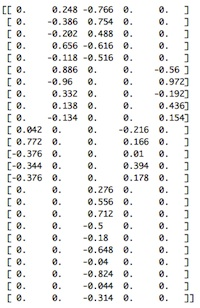
\includegraphics[natwidth=200, natheight=306]{m_img}
	\caption{Group-wise sparse weight matrix generated: 6 classes, 30 features in 5 groups}
\end{center}
\end{figure}

Then we generate random vectors, each of which has the length of the number of all features, and calculate dot product with the weight matrix M to get the class assignments for these random vectors. The random vetors X and the class assignments Y make up the training data set. \\

Our goal is to infer this weight matrix M from X and Y using our model. By generating the data set using this method, we can test the effectiveness of our model on a noiseless dataset with right underlying assumptions.\\ 


\section{Results}

\section{Conclusion}
% include your own bib file like this:
%\bibliographystyle{acl}
%\bibliography{acl2014}

%\begin{thebibliography}{}
%
%\bibitem[\protect\citename{Aho and Ullman}1972]{Aho:72}
%Alfred~V. Aho and Jeffrey~D. Ullman.
%\newblock 1972.
%\newblock {\em The Theory of Parsing, Translation and Compiling}, volume~1.
%\newblock Prentice-{Hall}, Englewood Cliffs, NJ.
%
%\bibitem[\protect\citename{{American Psychological Association}}1983]{APA:83}
%{American Psychological Association}.
%\newblock 1983.
%\newblock {\em Publications Manual}.
%\newblock American Psychological Association, Washington, DC.
%
%\bibitem[\protect\citename{{Association for Computing Machinery}}1983]{ACM:83}
%{Association for Computing Machinery}.
%\newblock 1983.
%\newblock {\em Computing Reviews}, 24(11):503--512.
%
%\bibitem[\protect\citename{Chandra \bgroup et al.\egroup }1981]{Chandra:81}
%Ashok~K. Chandra, Dexter~C. Kozen, and Larry~J. Stockmeyer.
%\newblock 1981.
%\newblock Alternation.
%\newblock {\em Journal of the Association for Computing Machinery},
%  28(1):114--133.
%
%\bibitem[\protect\citename{Gusfield}1997]{Gusfield:97}
%Dan Gusfield.
%\newblock 1997.
%\newblock {\em Algorithms on Strings, Trees and Sequences}.
%\newblock Cambridge University Press, Cambridge, UK.
%
%\end{thebibliography}

\end{document}
